\documentclass[12pt,letterpaper]{article}
\usepackage[margin=.63in,headheight=15pt,headsep=19pt,footskip=25pt]{geometry}
\usepackage{tikz,fancyhdr,array}
\usetikzlibrary{arrows.meta}
\renewcommand{\familydefault}{\sfdefault}
\pagestyle{fancy}\fancyhf{}\renewcommand{\headrulewidth}{.4pt}
\fancyhead[L]{\small Week 23 / Sorting machines encore / Grades 2--5}
\fancyfoot[L]{\small Bellingham Math Circle / Week 23 / W23-BON-v1}\fancyfoot[R]{\small\thepage}
\setlength{\parindent}{0pt}\setlength{\parskip}{9pt}
\newcommand{\problem}[2]{\textbf{Problem #1:} #2\par}
\newcommand{\lines}[1]{\foreach \i in {1,...,#1}{\par\vspace{10pt}\hrulefill}\par}
\newcommand{\blankfour}{\begin{tikzpicture}[x=1cm,y=18mm]\foreach \i in {1,2,3,4}{\node at (-.5,1-\i){\i};\draw[-{Stealth}] (0,1-\i)--(14,1-\i);}\end{tikzpicture}}
\newcommand{\machine}[3][1]{\begin{tikzpicture}[x=1cm,y=18mm,scale=#1]\foreach \i in {1,...,#2}{\node at (-.5,1-\i){\i};\draw[-{Stealth}] (0,1-\i)--(12,1-\i);}\foreach \x/\a/\b in {#3}{\draw[very thick] (\x,1-\a)--(\x,1-\b);\fill (\x,1-\a) circle (2.5pt);\fill (\x,1-\b) circle (2.5pt);}\end{tikzpicture}}
\begin{document}
Cards move from left to right. Each bar compares only its two dotted lanes and sends the smaller value to the lower-numbered lane. Ties stay put. Fix every bar before choosing an input; use the same bars for every input.

\problem{1}{Use cards 1, 2, 3, 4. Build a machine that always puts the smallest card in lane 1. The other lanes may be in any order. Find the fewest bars possible, and explain why fewer cannot work.}
\begin{center}\blankfour\end{center}
\begin{center}\renewcommand{\arraystretch}{2}\begin{tabular}{p{2.6in}|p{2.6in}}
input, in lane order&output, in lane order\\\hline
&\\\hline &\\\hline &\\\hline &\\\hline
\end{tabular}\end{center}
\lines{5}
\newpage
\problem{2}{Use cards 1, 2, 3, 4 in every possible input order. Does this machine always put the two smallest cards in lanes 1 and 2, in either order? Find an input whose output is not fully sorted. Explain the machine's guarantee.}
\begin{center}\machine{4}{1.5/1/2,4.5/3/4,7.5/1/4,10.5/2/3}\end{center}
\begin{center}\renewcommand{\arraystretch}{2}\begin{tabular}{p{2.6in}|p{2.6in}}
input, in lane order&output, in lane order\\\hline
&\\\hline &\\\hline &\\\hline &\\\hline &\\\hline
\end{tabular}\end{center}
\lines{5}
\newpage
For merging, lanes 1 and 2 begin as a sorted pair, and lanes 3 and 4 begin as a sorted pair. Keep the two pairs in their trays until the machine starts.

\problem{3}{Build a fixed machine that merges the two sorted pairs into one sorted output. Use the fewest bars you can. It must work for all six inputs below. Explain why fewer bars cannot work.}
\begin{center}\blankfour\end{center}
\begin{center}\renewcommand{\arraystretch}{1.6}\begin{tabular}{c|p{3in}}
lanes 1,2 / lanes 3,4&output, in lane order\\\hline
1,2 / 3,4&\\\hline 1,3 / 2,4&\\\hline 1,4 / 2,3&\\\hline
2,3 / 1,4&\\\hline 2,4 / 1,3&\\\hline 3,4 / 1,2&\\\hline
\end{tabular}\end{center}
\vspace{12pt}
\problem{4}{Give your three-bar merger an input whose pairs are not already sorted. Find an input that it fails to sort.}
\lines{3}
\newpage
Corner tags follow the cards and never take part in comparisons. Equal cards' order means their order by lane number, before and after the machine.

\begin{center}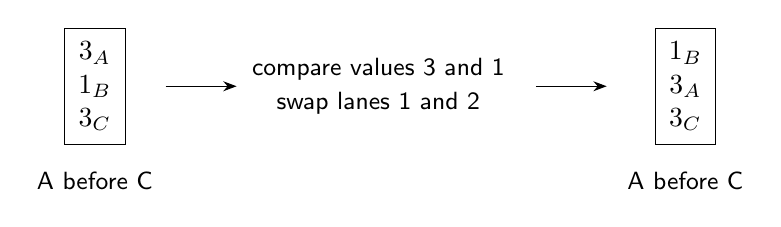
\begin{tikzpicture}[x=1cm,y=1cm]
\node[align=center,draw,inner sep=5pt] at (1,0){$3_A$\\$1_B$\\$3_C$};
\draw[-{Stealth}] (1.9,0)--(2.8,0);\node[align=center] at (4.6,0){\small compare values 3 and 1\\\small swap lanes 1 and 2};
\draw[-{Stealth}] (6.6,0)--(7.5,0);\node[align=center,draw,inner sep=5pt] at (8.5,0){$1_B$\\$3_A$\\$3_C$};
\node[font=\small] at (1,-1.2){A before C};\node[font=\small] at (8.5,-1.2){A before C};
\end{tikzpicture}\end{center}

\problem{5}{Use cards $2_A$, $2_B$, $1_C$ in all six input orders. Which machine keeps the two equal cards in their input order every time? Record the tagged outputs.}
\begin{center}\begin{minipage}{.48\textwidth}\centering\small machine X\par\machine[.52]{3}{2/1/3,6/1/2,10/2/3}\end{minipage}\hfill\begin{minipage}{.48\textwidth}\centering\small machine Y\par\machine[.52]{3}{2/1/2,6/2/3,10/1/2}\end{minipage}\end{center}
\begin{center}\renewcommand{\arraystretch}{1.6}\begin{tabular}{c|p{1.9in}|p{1.9in}}
input&machine X output&machine Y output\\\hline
$2_A,2_B,1_C$&&\\\hline $2_A,1_C,2_B$&&\\\hline $2_B,2_A,1_C$&&\\\hline
$2_B,1_C,2_A$&&\\\hline $1_C,2_A,2_B$&&\\\hline $1_C,2_B,2_A$&&\\\hline
\end{tabular}\end{center}
\problem{6}{A bar between neighboring lanes swaps no card over a third card. Can a machine made only from such bars ever reverse two equal cards? Explain.}
\lines{3}
\end{document}
